\clearpage
\begin{figure}[htp]
\begin{center}
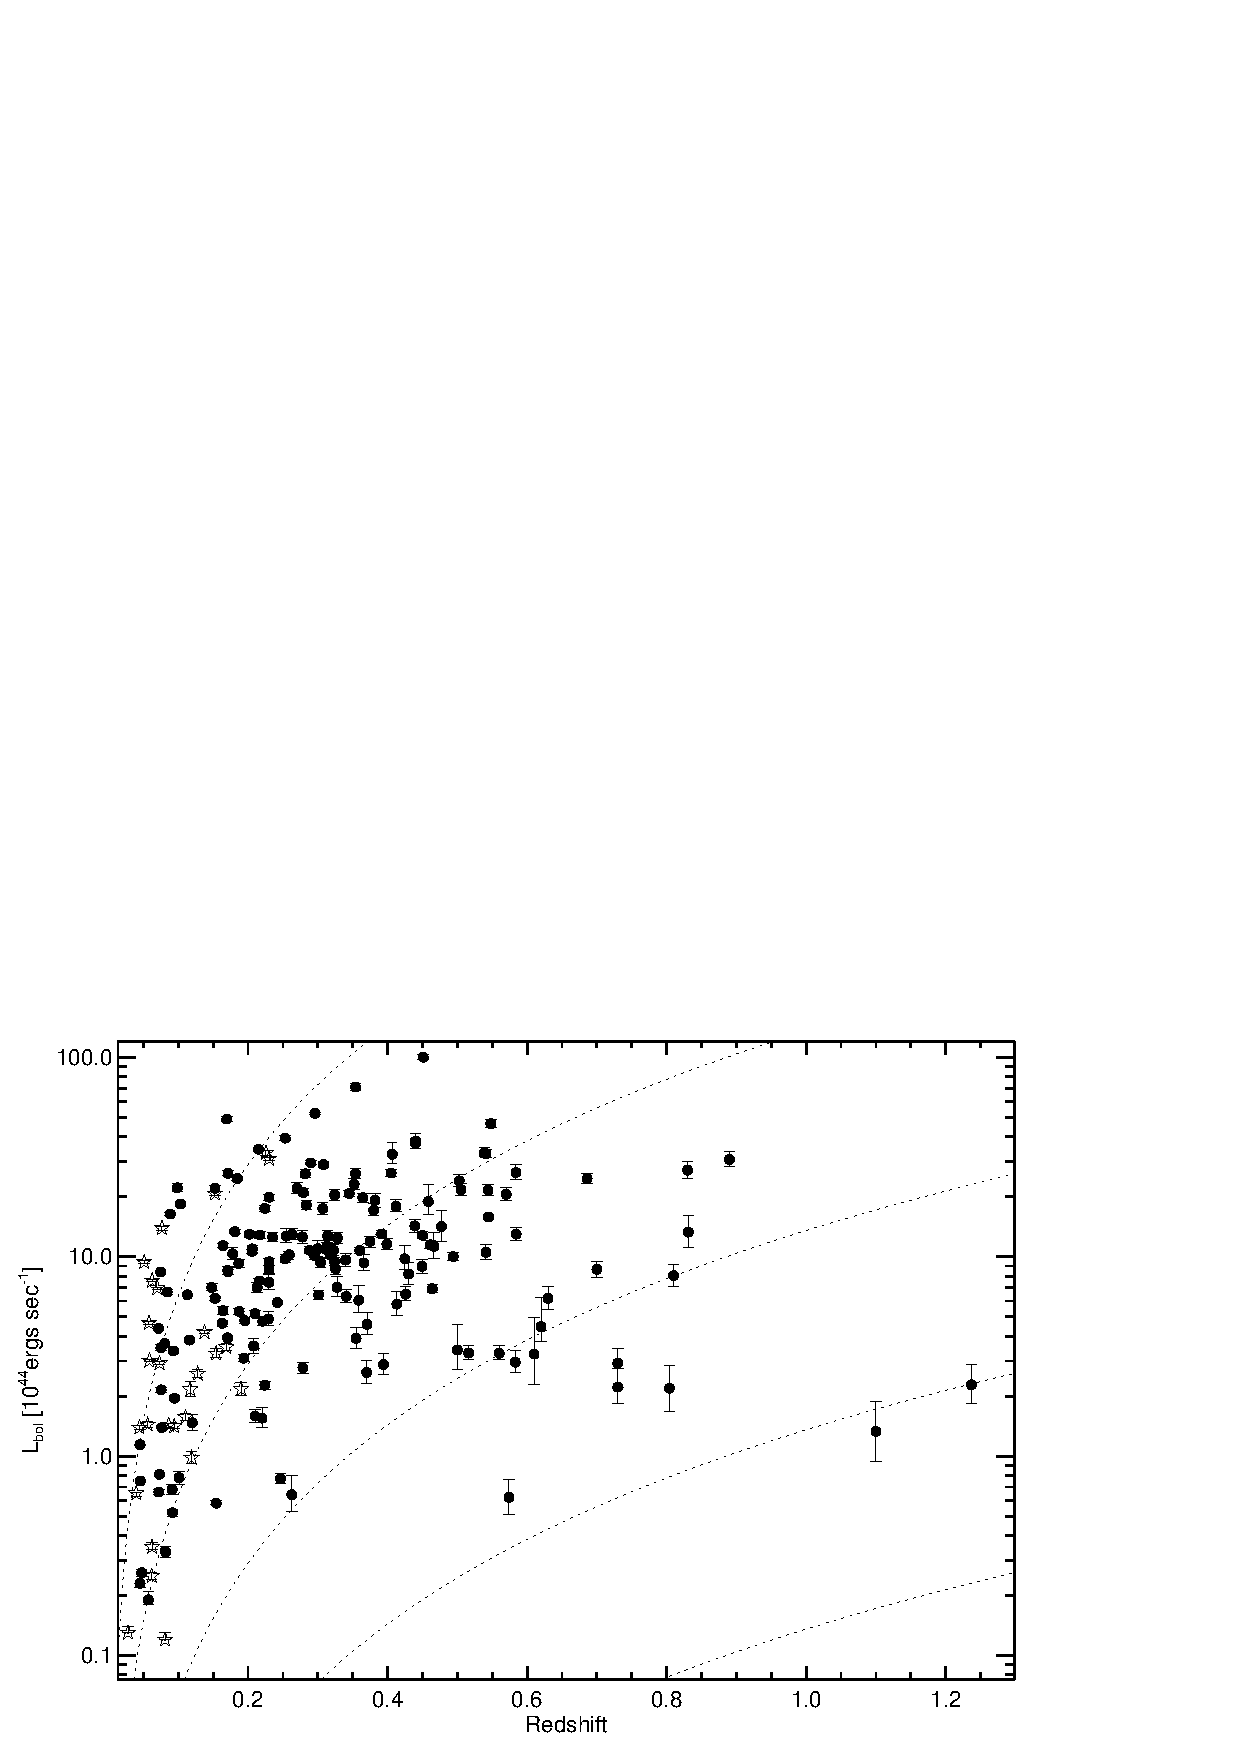
\includegraphics[scale=1.0]{lx_z}
\caption{\small
Bolometric luminosity ($E = 0.1-100$ keV) plotted as a function of
redshift for the full sample. $L_{bol}$ values are limited to the
region of spectral extraction $R=R_{2500-\mathrm{CORE}}$ (or
$R=R_{5000-\mathrm{CORE}}$ for clusters without $R_{2500-\mathrm{CORE}}$
fits). Dotted lines represent constant fluxes of $3.0\times10^{-15}$,
$10^{-14}$, $10^{-13}$, and $10^{-12}$ ergs sec$^{-1}$ cm$^{-2}$.
}
\label{fig:lx_z}
\end{center}
\end{figure}

\clearpage
\begin{figure}[htp]
\begin{center}
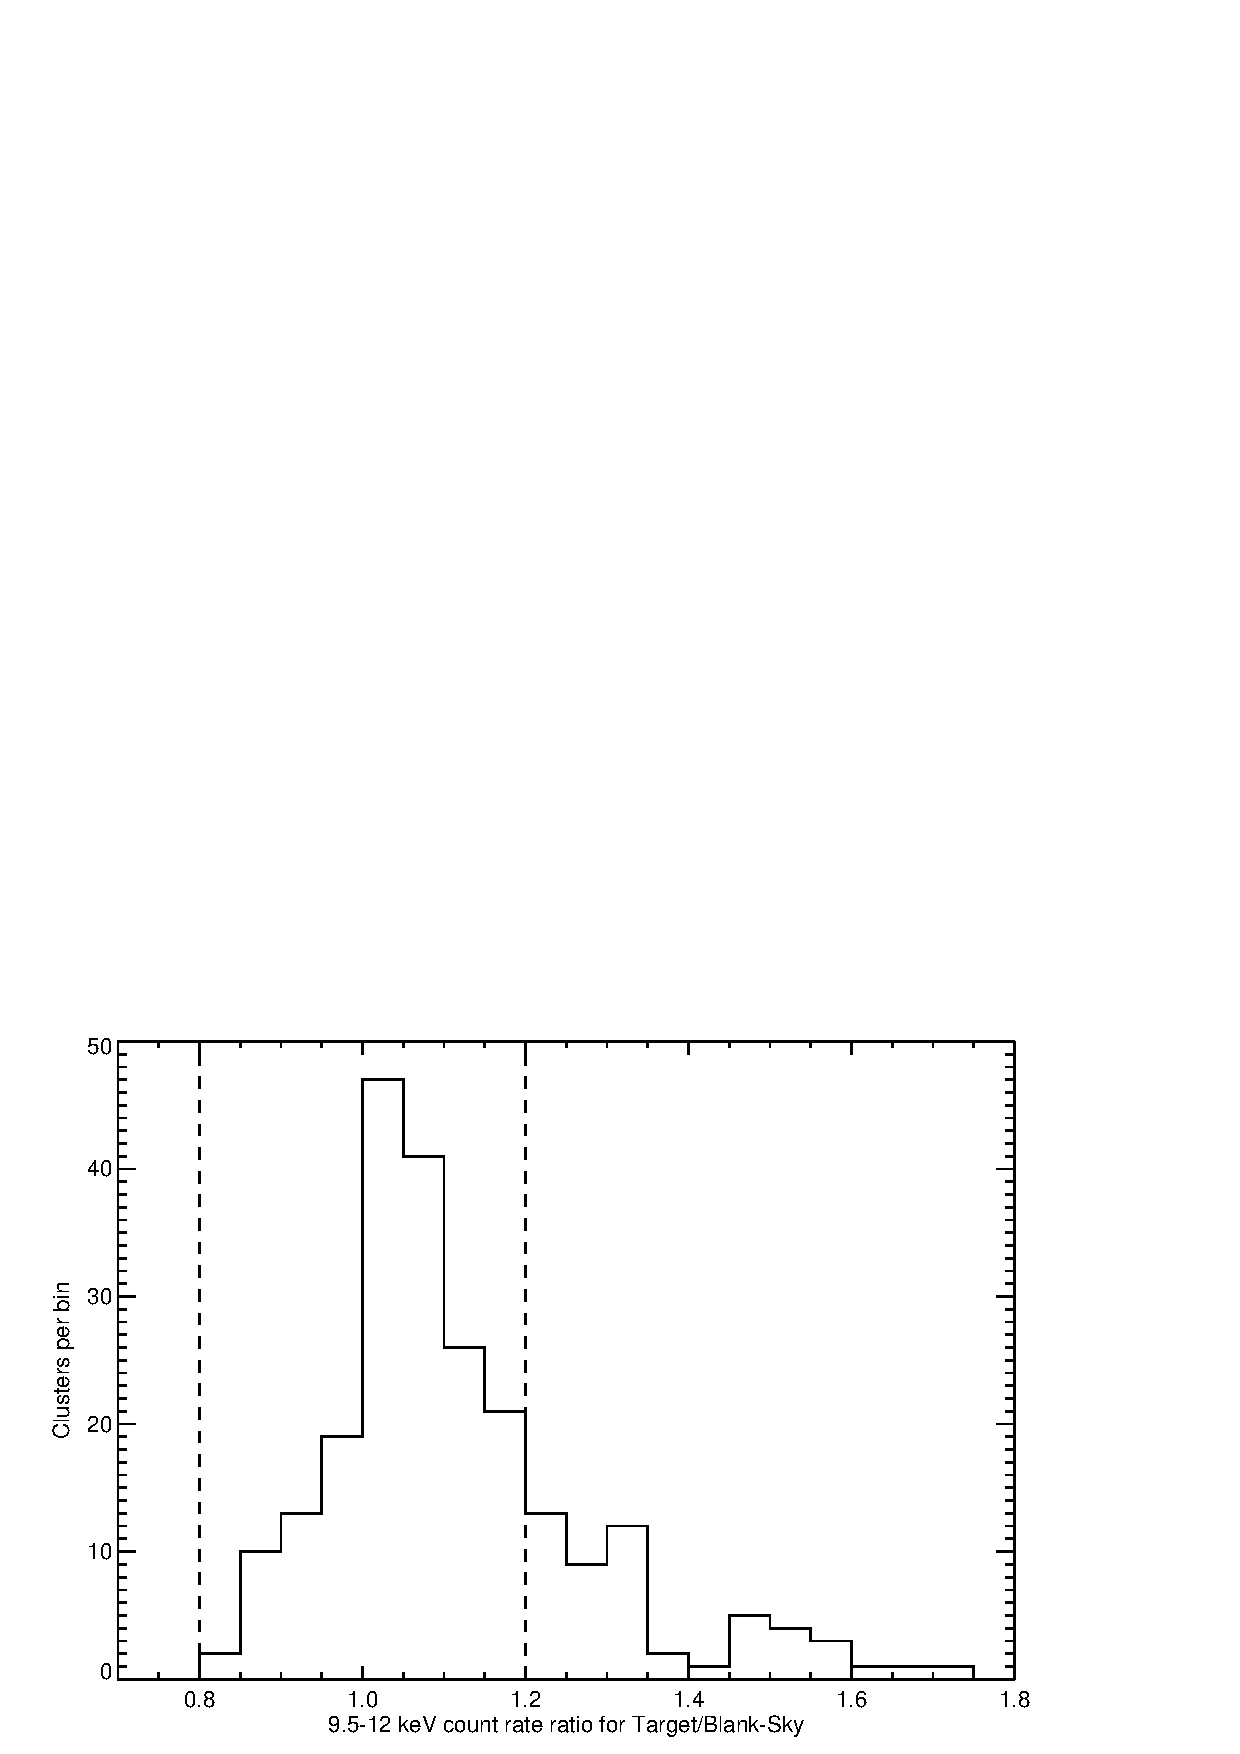
\includegraphics[scale=1.0]{bgd_fig}
\caption{\small
Ratio of target field and blank-sky field count rates in the 9.5-12.0
keV band for each observation. Vertical dashed lines represent $\pm
20\%$ of unity.
}
\label{fig:bgd}
\end{center}
\end{figure}

\clearpage
\begin{figure}[htp]
\begin{center}
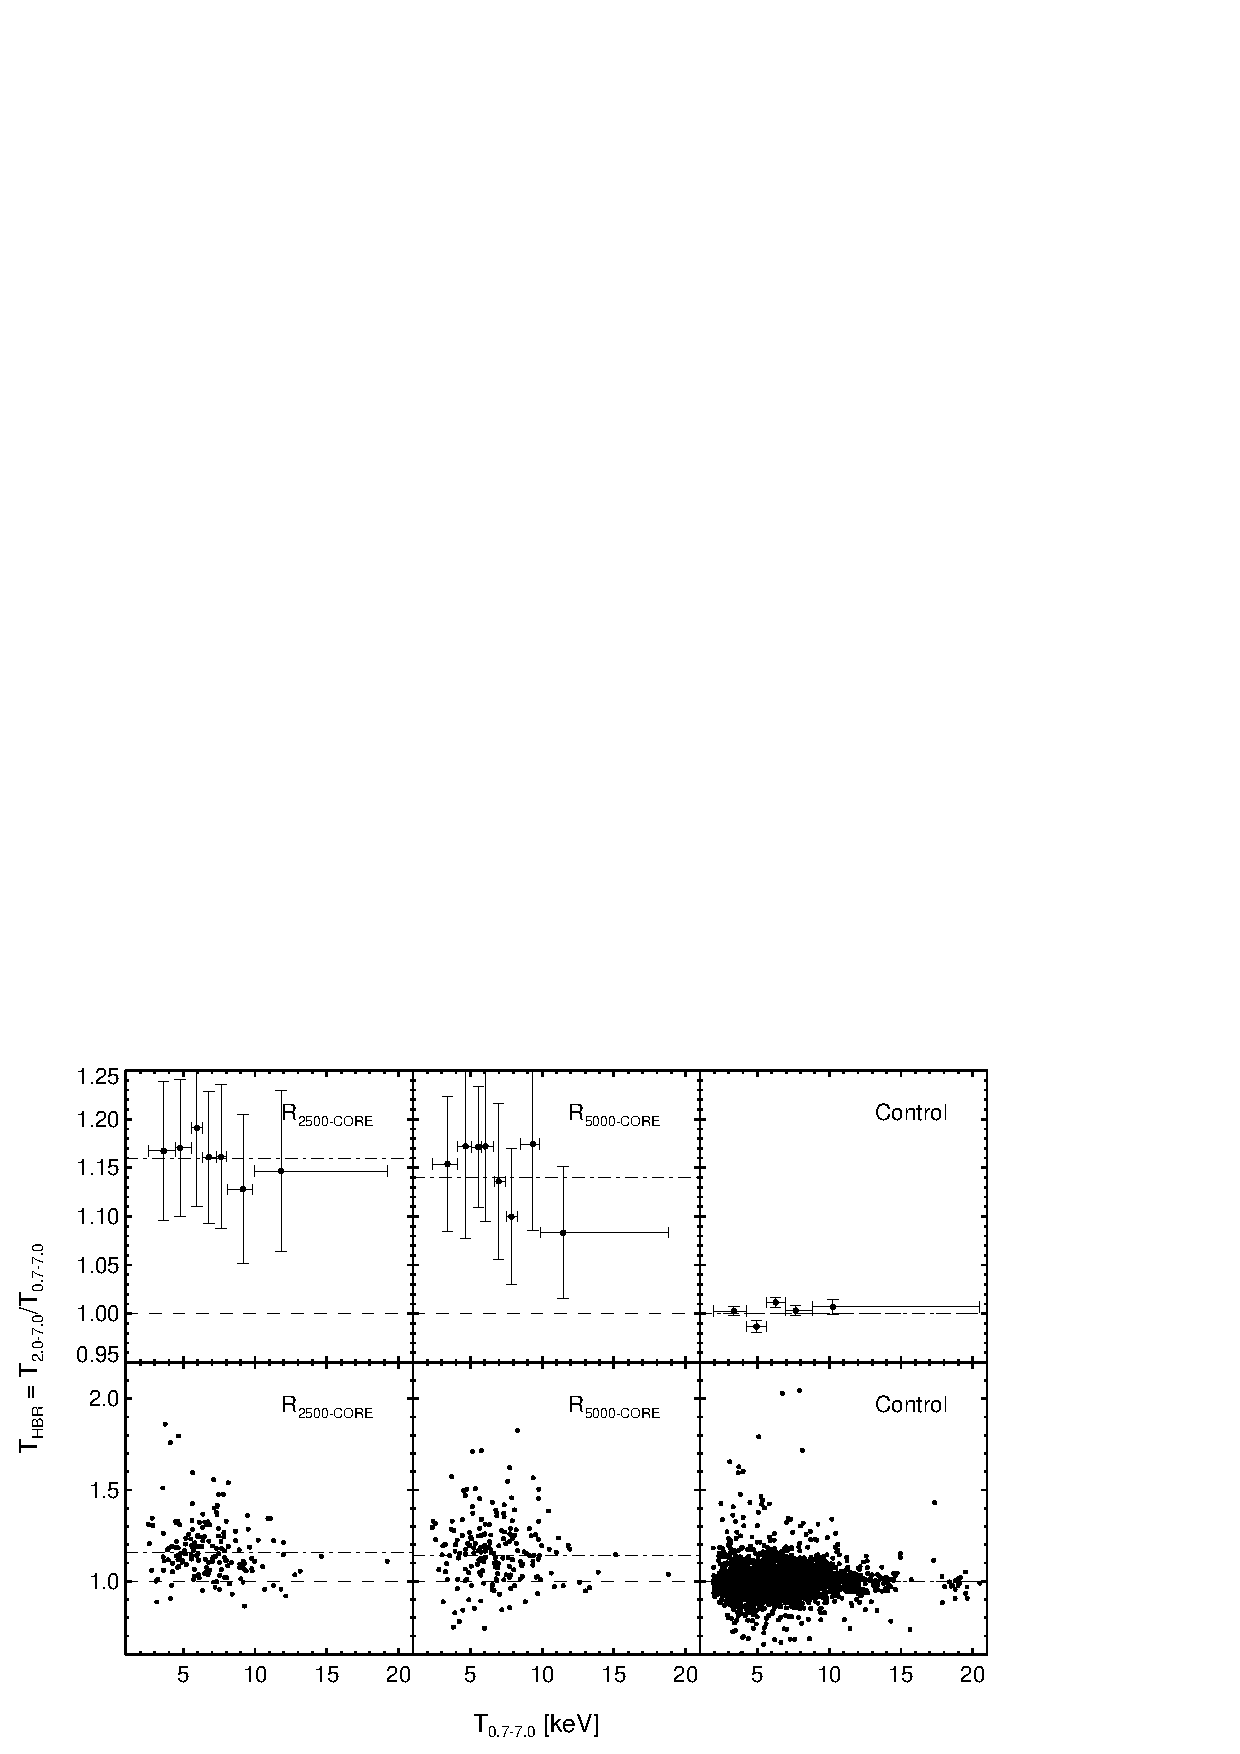
\includegraphics[scale=1.0]{ftxcount}
\caption{\small
Best-fit temperatures for the hard-band, $T_{2.0-7.0}$, divided by the
broad-band, $T_{0.7-7.0}$, and plotted against the broad-band
temperature. For binned data, each bin contains 25 clusters, with the
exception of the highest temperature bins which contain 16 and 17 for
$R_{2500-\mathrm{CORE}}$ and $R_{5000-\mathrm{CORE}}$, respectively. The
simulated data bins contain 1000 clusters with the last bin having 780
clusters. The line of equality is shown as a dashed line and the
weighted mean for the full sample is shown as a dashed-dotted
line. Error bars are omitted in the unbinned data for clarity. Note
the net skewing of $T_{HBR}$ to greater than unity for both apertures
with no such trend existing in the simulated data. The dispersion of
$T_{HBR}$ for the real data is also much larger than the dispersion of
the simulated data.
}
\label{fig:ftx}
\end{center}
\end{figure}

\clearpage
\begin{figure}[htp]
\begin{center}
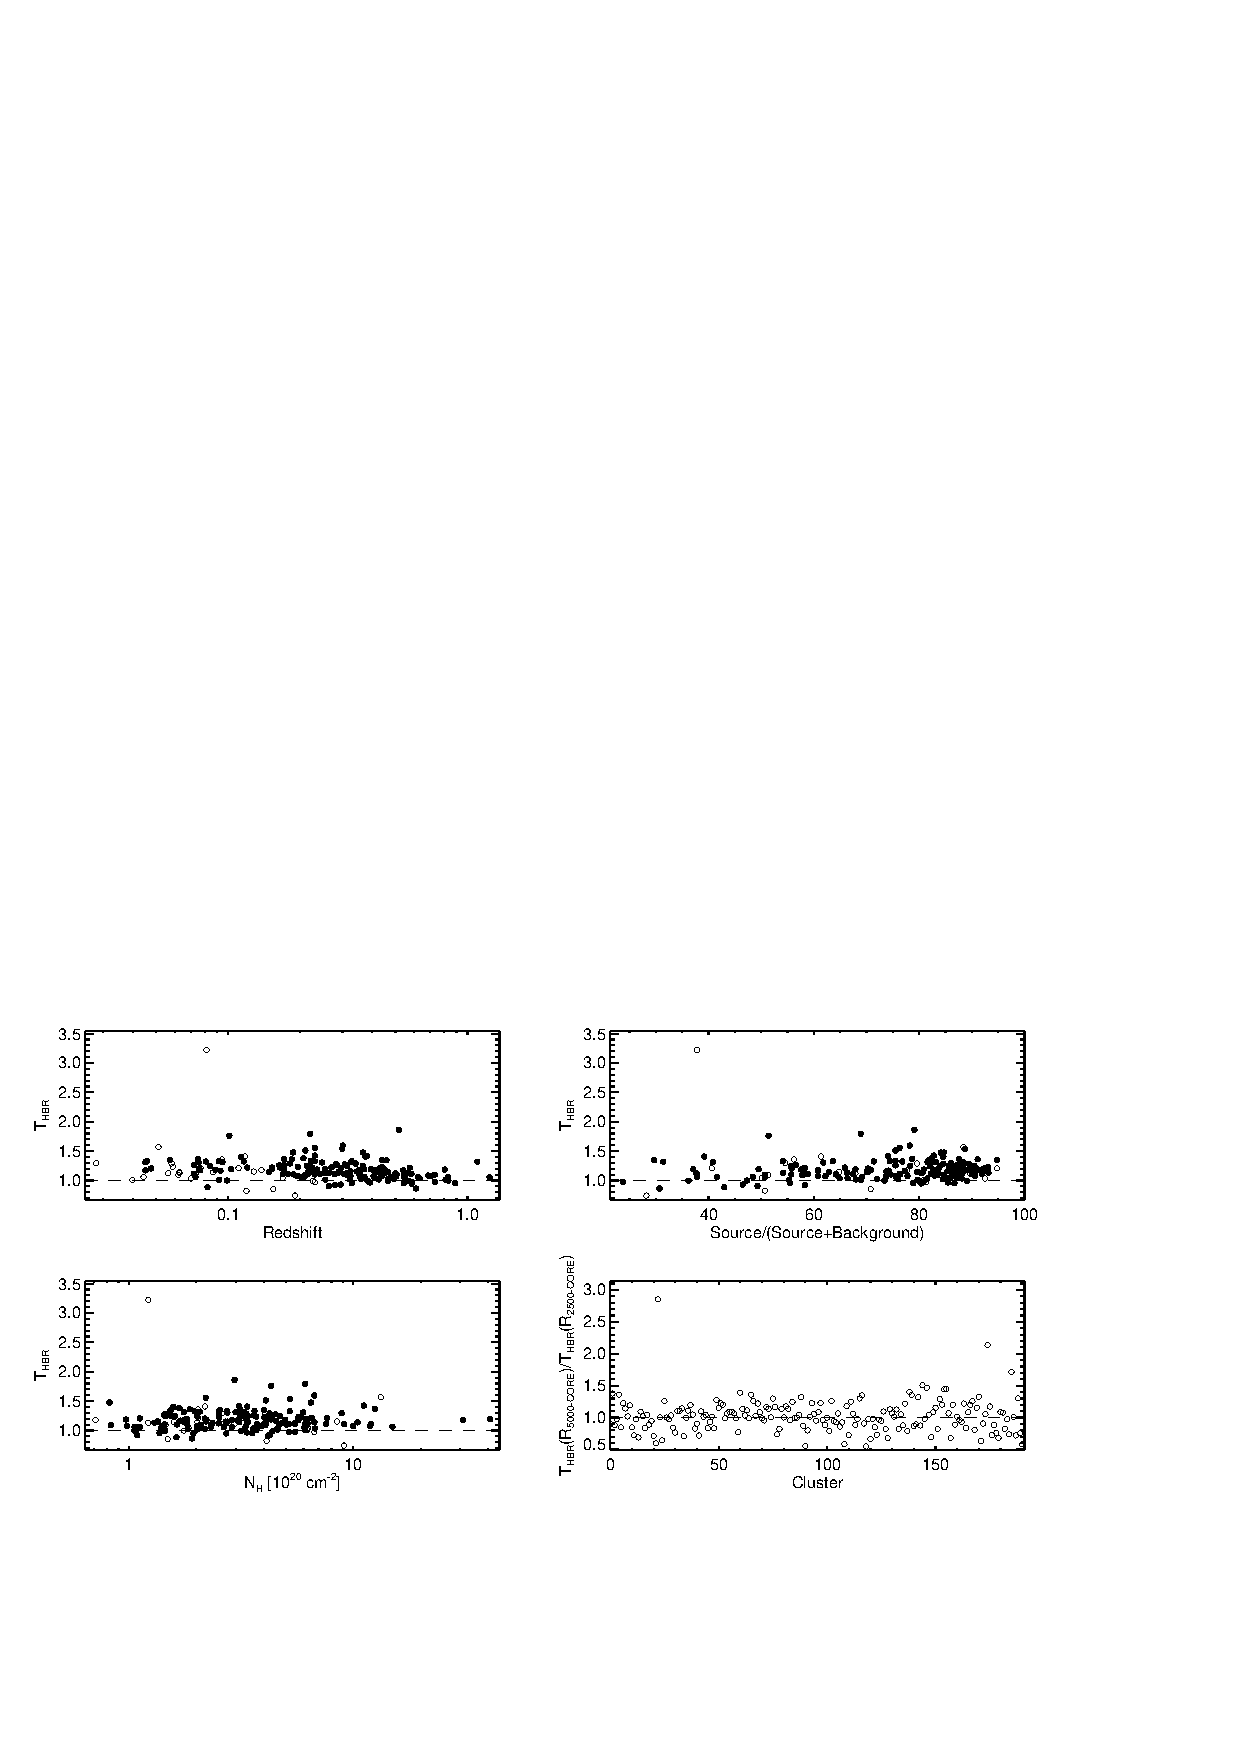
\includegraphics[scale=1.0]{sys}
\caption{\small
Plotted here are a few possible sources of systematic uncertainty.
Error bars have been omitted in all plots for clarity. The line of
equality is shown as a dashed line in all
plots. {\bfseries\em{(Upper-left:)}} $T_{HBR}$ versus redshift for the
entire sample. The trend in $T_{HBR}$ with redshift is expected as the
$T_{2.0-7.0}$ lower boundary nears convergence with the $T_{0.7-7.0}$
lower boundary at $z \approx 1.85$. Weighted values of $T_{HBR}$ are
consistent with unity starting at $z \sim
0.6$. {\bfseries\em{(Upper-right:)}} $T_{HBR}$ versus percentage of
spectrum flux which is attributed to the source. We find no trend with
signal-to-noise which would suggest calibration uncertainty is playing
a major role in our results. {\bfseries\em{(Middle-left:)}} $T_{HBR}$
versus Galactic column density. We find no trend in absorption which
would result if $N_{HI}$ values are inaccurate or if we had improperly
accounted for local soft
contamination. {\bfseries\em{(Middle-right:)}} Ratio of $T_{HBR}$ for
our two physically motivated apertures, $R_{2500-\mathrm{CORE}}$ and
$R_{5000-\mathrm{CORE}}$. Error bars are omitted for clarity as they all
cross the line of equality. Different sized apertures do not result in
significantly different values of $T_{HBR}$ which indicates $T_{HBR}$
is insensitive to our definition of aperture
size. {\bfseries\em{(Lower-left:)}} $T_{HBR}$ plotted versus
observation start date. The plotted points are culled from the full
sample and represent only clusters which have a single observation and
where the spectral flux is $> 75\%$ from the source. We note no
systematic trend with time which suggests any contamination of {\it
Chandra}'s HRMA may not be changing with
time. {\bfseries\em{(Lower-right:)}} Ratio of {\it Chandra}
temperatures derived in this work to {\it ASCA} temperatures taken
from Don Horner's thesis. We note a trend of comparatively hotter {\it
Chandra} temperatures for clusters $> 10$ keV, otherwise our derived
temperatures are in good agreement with those of {\it ASCA}.
}
\label{fig:sys}
\end{center}
\end{figure}

\clearpage
\begin{figure}[htp]
\begin{center}
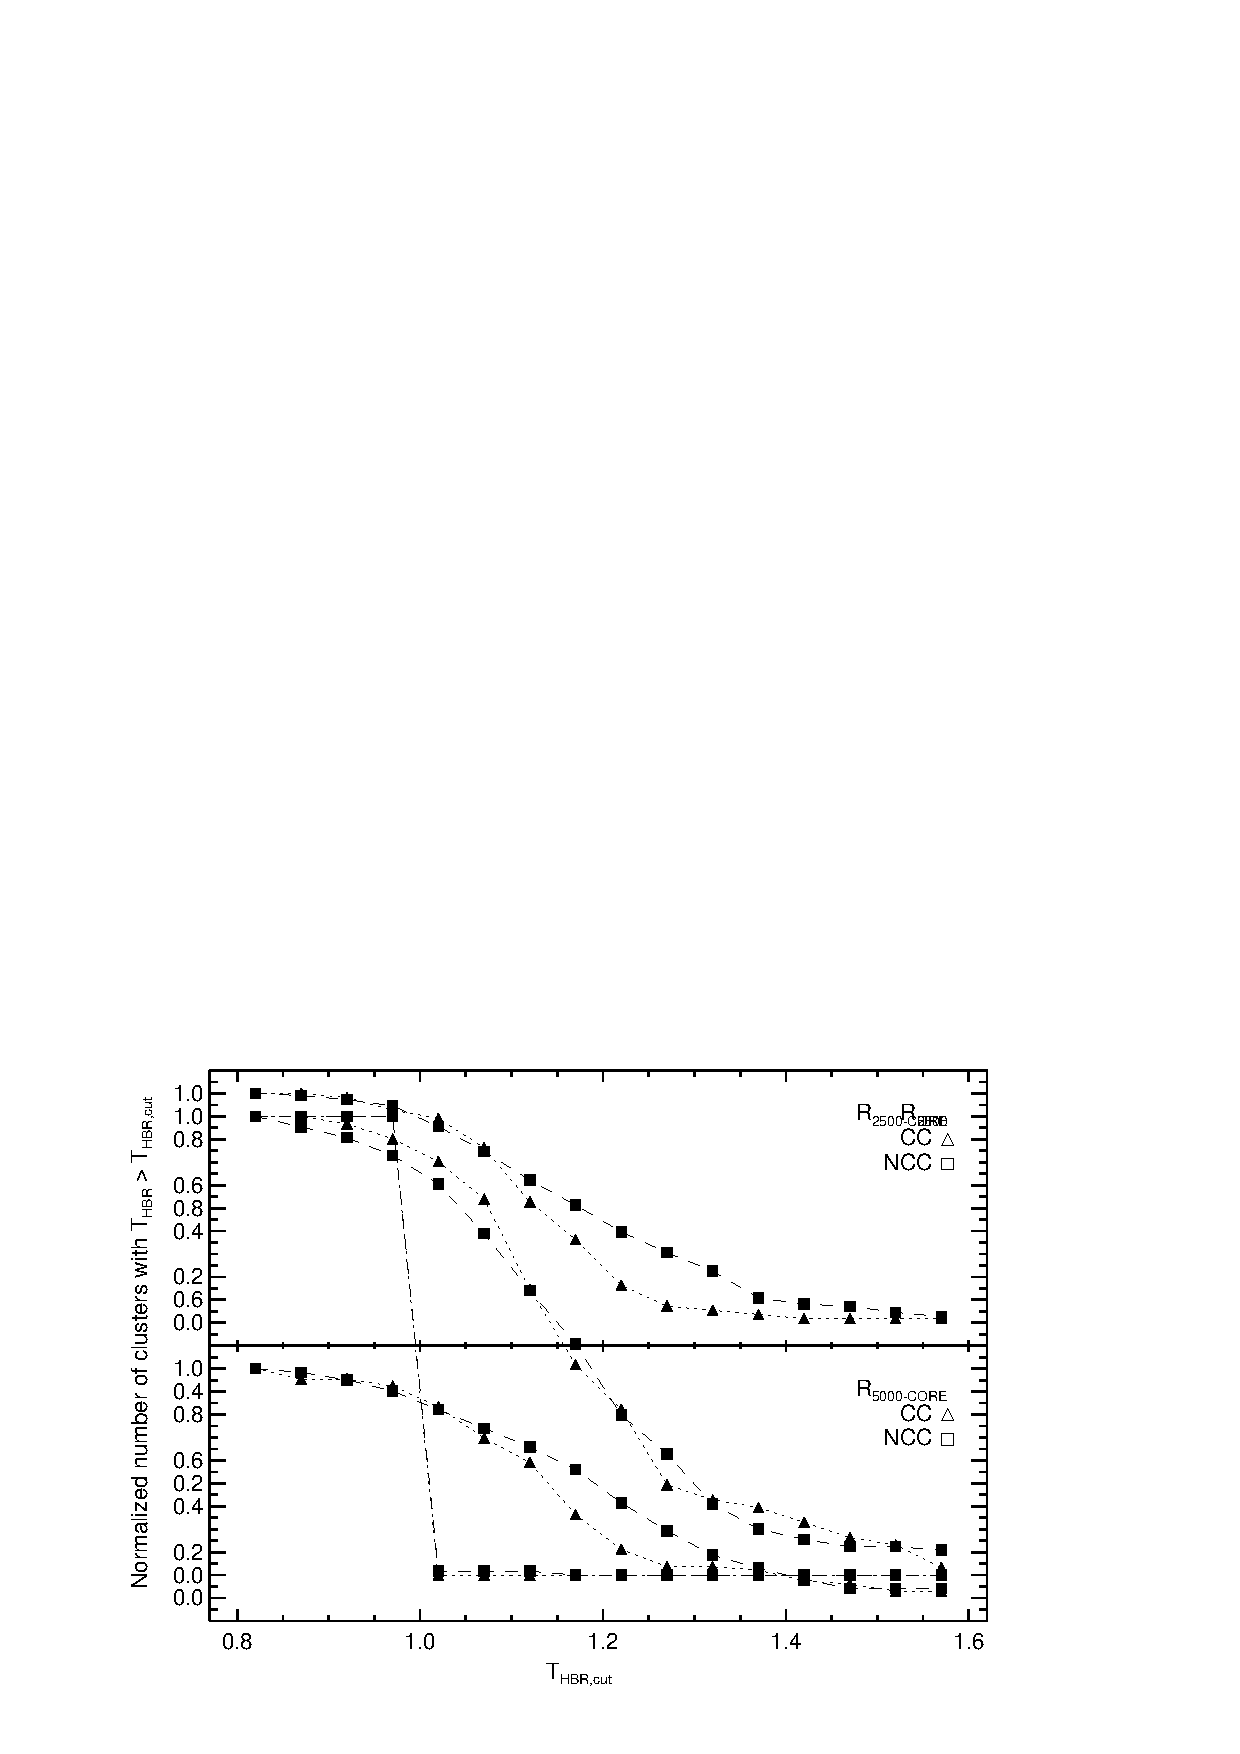
\includegraphics[scale=1.0]{cc_ncc_bin}
\caption{\small
Plotted here is the normalized number of cool core (CC) and non-cool core
(NCC) clusters as a function of cuts in $T_{HBR}$. We have defined a
cluster as having a cool core (CC) when the temperature for the 50 kpc
region around the cluster center divided by the temperature for
$R_{2500-\mathrm{CORE}}$ is less than 1 at the $2\sigma$ level. We then
take cuts in $T_{HBR}$ at the $1\sigma$ level and ask how many CC and
NCC clusters are above these cuts. The number of CC clusters falls off
more rapidly than NCC clusters in this classification scheme
suggesting higher values of $T_{HBR}$ prefer less relaxed systems
which do not have cool cores. This result is insensitive to our choice
of significance level in both the CC classification and $T_{HBR}$
cuts.
}
\label{fig:cc_ncc_bin}
\end{center}
\end{figure}

\clearpage
\begin{figure}[htp]
\begin{center}
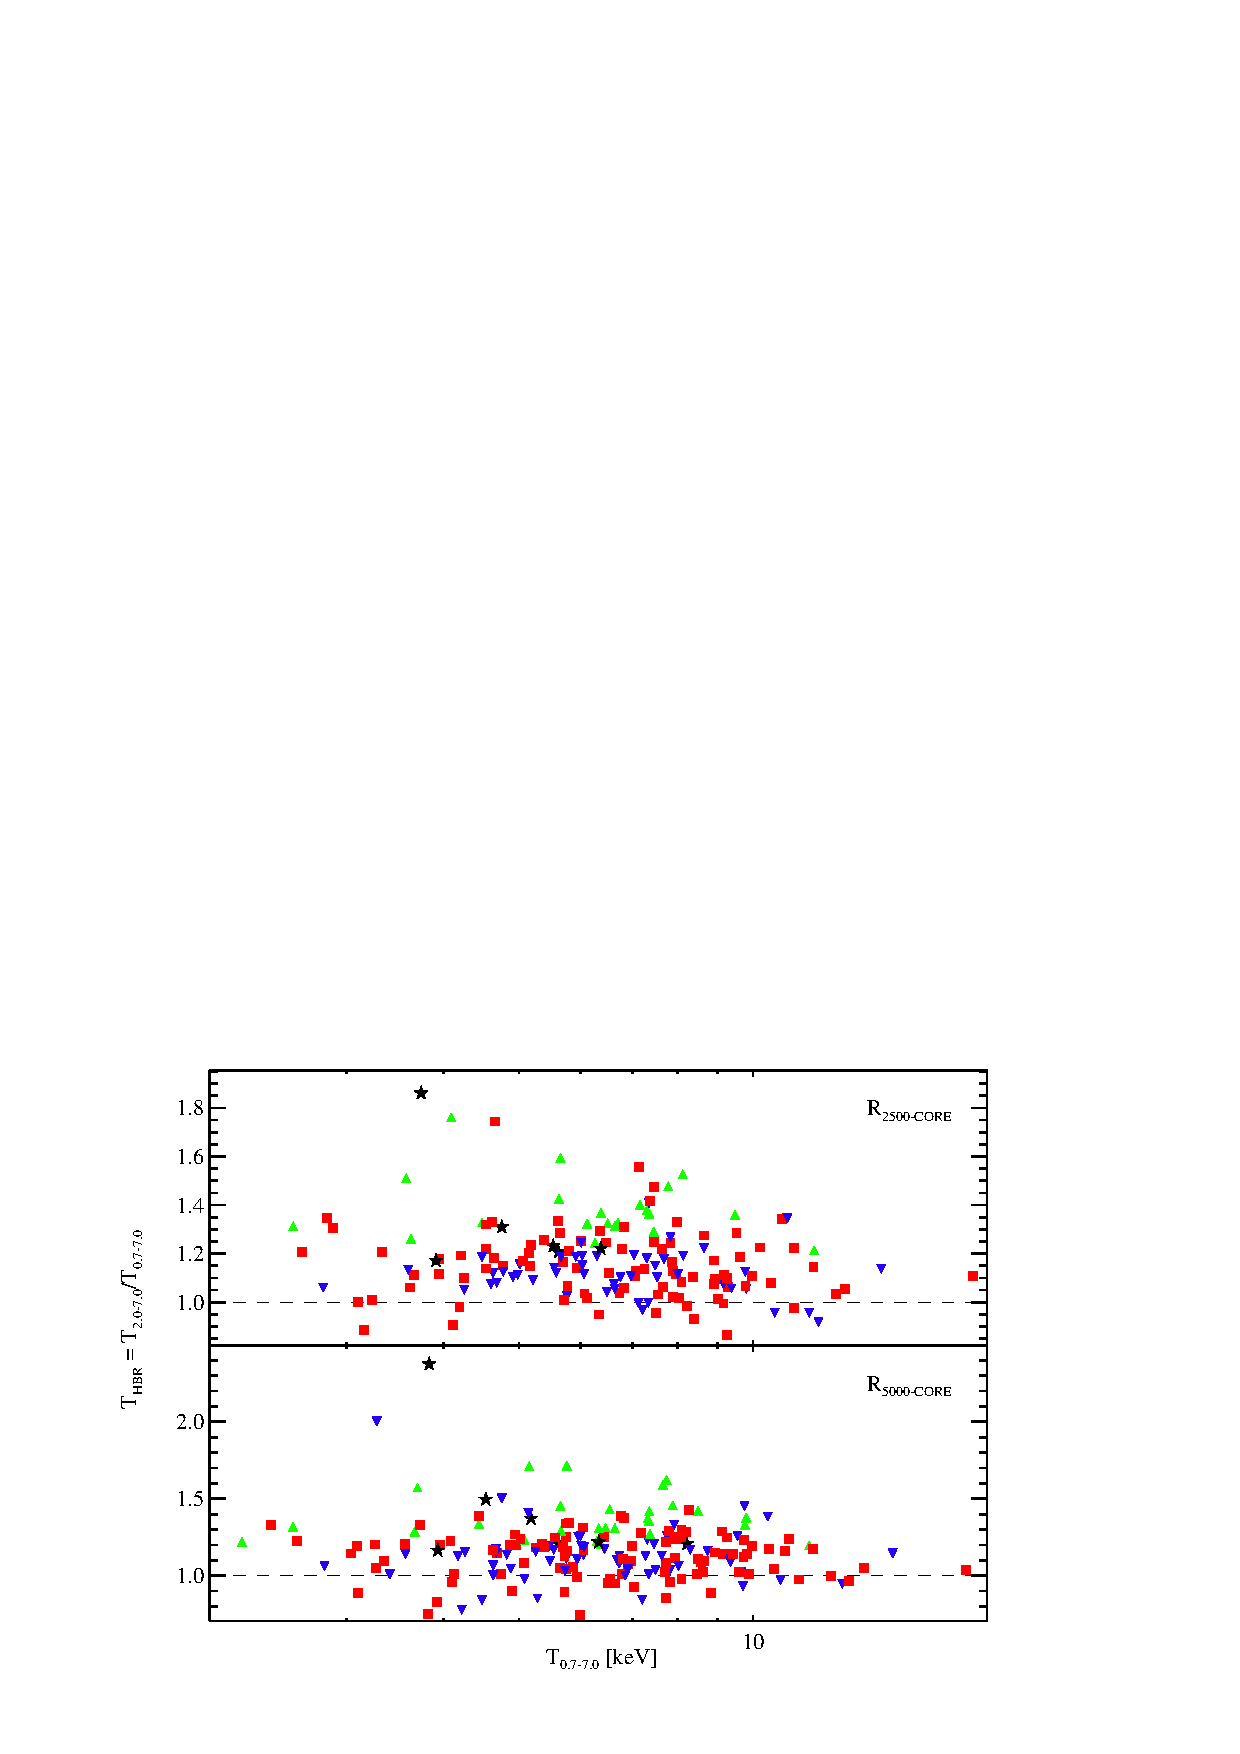
\includegraphics[scale=1.0]{ftx_tx_color}
\caption{\small
$T_{HBR}$ plotted against $T_{0.7-7.0}$ for our sample. Symbols and
color coding are based on two criteria: 1) presence of a cool core
(CC) and 2) value of $T_{HBR}$ value. Black stars are clusters with a
CC and $T_{HBR}$ significantly greater than 1.1. Green
upright-triangles are NCC clusters with $T_{HBR}$ significantly
greater than 1.1. Blue down-facing triangles are CC clusters and red
squares are NCC clusters. We have found most, if not all, of the
clusters with $T_{HBR} \gtrsim 1.1$ are merger systems. Note that the
cut at $T_{HBR} > 1.1$ is arbitrary and there are more merger systems
in our sample then just those highlighted in this figure. However it
is rather suggestive that clusters with the highest values $T_{HBR}$
share a common dynamic state.
}
\label{fig:ftx_tx}
\end{center}
\end{figure}
